\documentclass[11pt]{article} %Tipo de documento
%Tamaño de la hoja y tamaño de la fuente
\usepackage[utf8]{inputenc} % Codificación del texto
\usepackage[spanish]{babel} %Idioma del documento
%Luego estas
\usepackage{graphicx} %Inserción de imagenes
\usepackage{float} %Ajuste de figuras y tablas
\usepackage{subcaption} 
%Después estás
\usepackage{amsmath, amssymb,amsfonts}
%Finalmente éstas
\usepackage{apacite}


%Cuerpo del documento
\begin{document}
    

    \begin{figure}
        %Subfloat permitirá insertar las imágenes en el mismo lado
        \subfloat{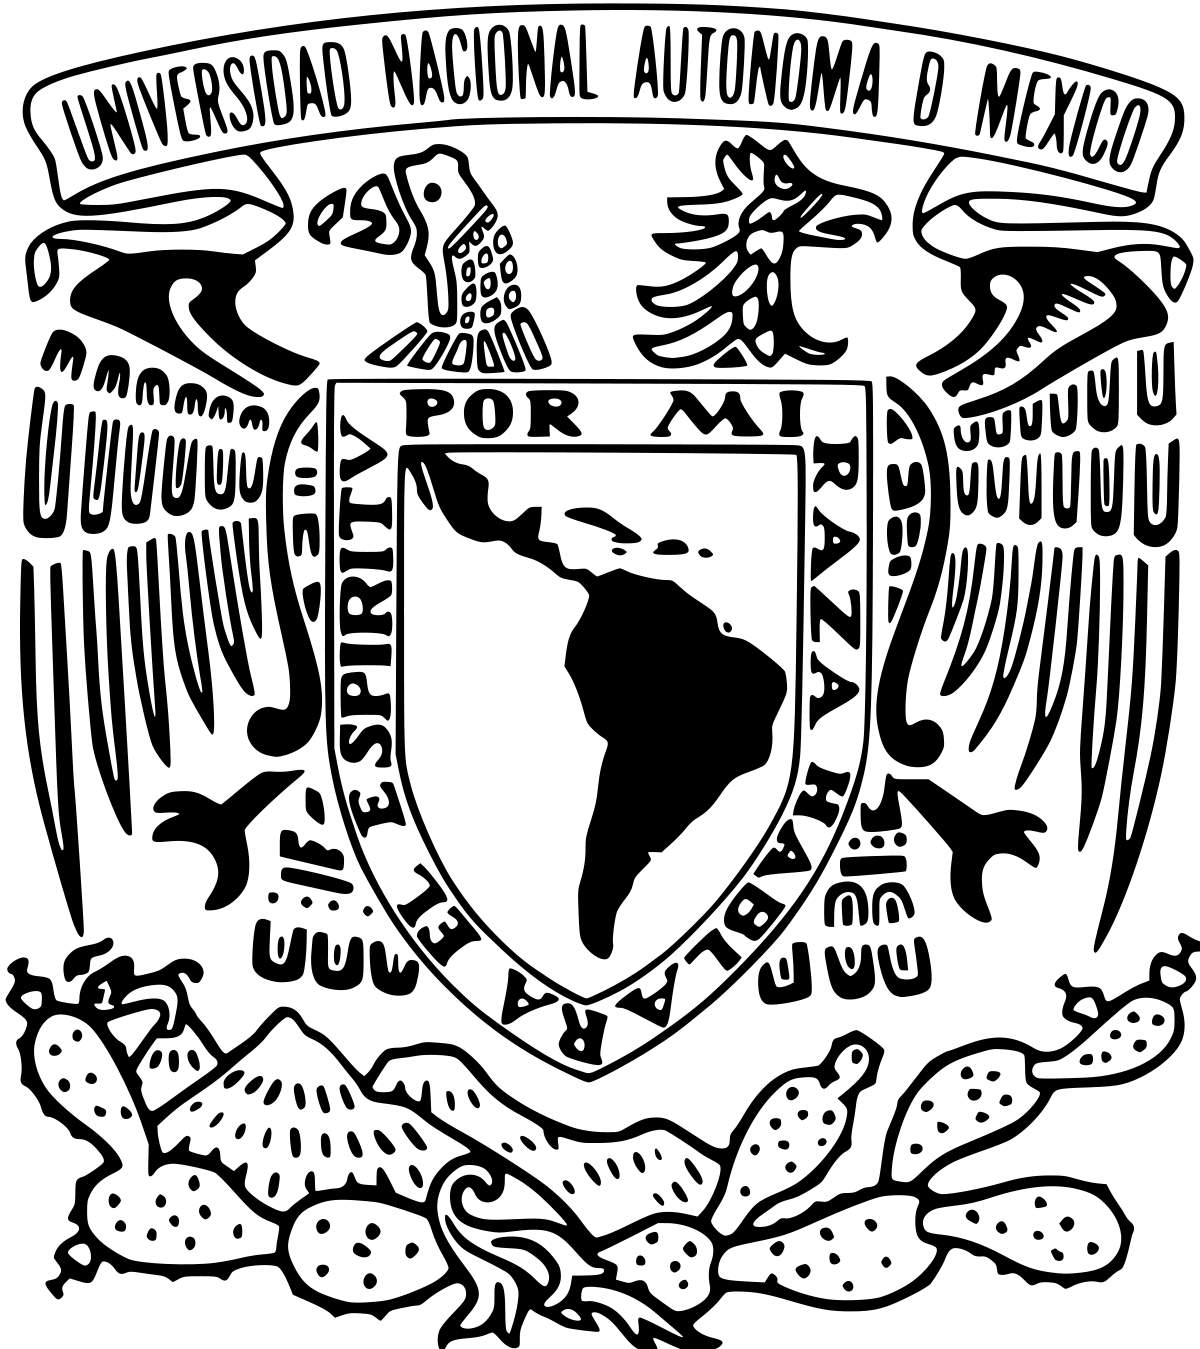
\includegraphics[width=0.2\textwidth]{unamescudo.png}}
        \hfill
        \subfloat{
\includegraphics[width=0.2\textwidth]{escudofi_negro}}
    \end{figure}
    

    \vspace{1cm}

    %Cuerpo de la portada 
    \begin{titlepage}                     
        \centering
        {\bfseries\LARGE Universidad Nacional Aut\'onoma de M\'exico \par}
        \vspace{1cm}
        {\bfseries\LARGE Facultad de Ingenier\'ia \par}
        \vspace{1cm}
        {\bfseries\LARGE Divisi\'on de Ingenier\'ia El\'ectrica\par}
        \vspace{1cm}
        {\itshape\Large \textbf{Materia o curso\\} \par} 
        \vspace{1cm}
        {\scshape\Huge{Nombre del trabajo\\} \par}
        \vspace{1cm}
        {\itshape\Large \textbf{Nombre del o la docente que imparte el curso\\} \par}
        \vspace{1cm}
        \vfill
        {\itshape\Large Autor \\\par}
        \vfill
        \vspace{1cm}
        {\itshape\Large \today\par}   
    \end{titlepage}
	
    \newpage

     %%%%%%%%%%%%%%%%%%%%%%%%%%%%%%%%%%%%%%%%%%%%%%%%%%%%%%%%%%%%%%%%%%%%
     \newpage
     \section*{1.Objetivo}
         \Large{Desarrollar una plantilla elemental en \LaTeX}
     
     %%%%%%%%%%%%%%%%%%%%%%%%%%%%%%%%%%%%%%%%%%%%%%%%%%%%%%%%%%%%%%%%%%%%   
     \section*{2. Introducción}
         \Large{Esto es un ejemplo, {\tiny aquí se mostrará el tamaño más pequeño de texto en \LaTeX} y también \textsc{diferentes estilos de fuente}}. Existe una {\huge gran variedad de tamaños} para tu documento.
     
     %%%%%%%%%%%%%%%%%%%%%%%%%%%%%%%%%%%%%%%%%%%%%%%%%%%%%%%%%%%%%%%%%%%%
     \section*{3. Posicionamiento de im\'agenes}
         \subsection*{3.1 Armado y simulación de circuito}
         Se realizó la simulación del siguiente circuito y el espectro de magnitud, utilizando el analizador de frecuencias.
         %%%%%%%%%%%%%%%%%% IMAGEN 1 %%%%%%%%%%%%%%%%%% 
         \begin{figure}[htbp]
             \centering
             \includegraphics[width=0.60\textwidth]{REPORTE_IMAGEN_E1.jpeg}
             \caption{Circuito 1}
         \end{figure}
         
         %%%%%%%%%%%%%%%%%% IMAGEN 2 %%%%%%%%%%%%%%%%%% 
         \begin{figure}
             \centering
             {\includegraphics[width=0.60\textwidth]{REPORTE_IMAGEN_E1.jpeg}}
             \caption{Circuito 1}
         \end{figure}
         
         %%%%%%%%%%%%%%%%%% IMAGEN 3 %%%%%%%%%%%%%%%%%% 
         \begin{figure}
             \centering
             {\includegraphics[width=0.60\textwidth]{REPORTE_IMAGEN_E1_3.jpeg}}
             \caption{Resultado obtenido del circuito 1.}
         \end{figure}
     
         %%%%%%%%%%%%%%%%%% IMÁGENES JUNTAS %%%%%%%%%%%%%%%%%% 
    
         \begin{figure} 
             \centering
             \begin{subfigure}{0.45\textwidth}
                  \includegraphics[width=\textwidth]{REPORTE_IMAGEN_E1.jpeg}
                 \caption{Circuito}
             \end{subfigure}
             \hspace{1cm}
             \begin{subfigure}{0.45\textwidth}
                 \includegraphics[width=\textwidth]{REPORTE_IMAGEN_E1_3.jpeg}
                 \caption{Resultado}
             \end{subfigure}
             \caption{Experimento 1}
         \end{figure}
         
         
         
      %%%%%%%%%%%%%%%%%%%%%%%%%%%%%%%%%%%%%%%%%%%%%%%%%%%%%%%%%%%%%%   
     \section*{4. Inserci\'on de f\'ormulas matem\'aticas}
     
     \subsection*{4.1 Ecuaciones}
     %%Se pueden poner ecuaciones en medio de los símbolos de \$\$
     
     $\int f(x) \cdot dx$\\[3mm]
     $	a x^3 + b x^2 + c x + d = 0 $

     %O con el entorno equation
         \begin{equation} 
             a_{0}=\frac{1}{L}\int_{-L}^{L}f(x)dx 
             \label{FFT_2}
        \end{equation}
         %\centering
        
             El valor es 3 $V_{RMS}$\\
             $\text{La Fórmula Cuadrática es }x = \frac {-b \pm \sqrt {b^2 - 4ac}}{2a}$
         
             \begin{equation}
                 \text{La Fórmula Cuadrática es }x = \frac {-b \pm \sqrt {b^2 - 4ac}}{2a}
             \end{equation}
     %%%%%%%%%%%%%%%%%%%%%%%%%%%%%%%%%%%%%%%%%%%%%%%%%%%%%%%%%%%%%%%%%
     \subsection*{4.2 Exponenciaci\'on y radicaci\'on}
         \begin{equation}
             f=\frac{1}{T}=\frac{1}{2\times10^{-3}}=500Hz
             \label{ec_FFT}
         \end{equation}
         
         \begin{equation}
             FCresta=\frac{V_{pico}}{V_{RMS}}=\frac{4.24}{2.998}=1.4142\approx \sqrt{2} 
             \label{E3_fc}
         \end{equation}
         
         \begin{equation}
             f(x)=\frac{a_{0}}{2} + \sum_{n=1}^{\infty} a_{n}cos(\frac{n\pi x}{L}) +\sum_{n=1}^\infty b_{n}sen(\frac{n\pi x}{L})
             \label{ec_FFT1}
     \end{equation}
     %%%%%%%%%%%%%%%%%%%%%%%%%%%%%%%%%%%%%%%%%%%%%%%%%%%%%%%%%%%
     \section*{4.3 Funciones trigonom\'etricas}
         \begin{equation}
             A\sin(\alpha)+B\sin(\beta)
             \label{ec_superposicion}
         \end{equation}
         
         \begin{equation} 
             a_{n}=\frac{1}{L}\int_{-L}^{L}f(x)cos(\frac{n\pi x}{L})dx 
             \label{FFT_3}
        \end{equation}

     \section*{5. Inserci\'on de bibliograf\'ia}
     
     \textbf{Cita de un libro}
     Gaona define un algorimo de la siguiente palabra: ``Es la especificaci\'on de los datos y la descripci\'on
     de los pasos que deben seguirse para resolverse un problema" \cite{C1}
     
     \textbf{Cita de un artículo}\\
     Extraño - desconocido. Percibimos al otro, pero no fomentamos un acercamiento. Sólo vemos aspectos físicos, externos, y descriptivos. \cite{C2}
     
     \newpage

\bibliographystyle{apacite}
\bibliography{bibliografia.bib}        
\end{document}